\section{Component View}
\subsection{Database}
The database tier runs MySQL Community Edition and uses InnoDB as storage engine: the DBMS is fully transactional with rollback and commit,besides it ensure ACID properties and provides automatic recovery from crashes via the replay of logs. The DBMS will not be internally designed because it is an external component used as a “black box” offering some services: it only needs to be configured and tuned in the implementation phase. The database can communicate only with the business logic tier using the standard network interface, described in section 2.6. Security restrictions will be implemented to protect the data from unauthorized access: the database must be physically protected and the communication has to be encrypted. Access to the data must be granted only to authorized users possessing the right credentials and system privileges allow only administrators to perform administrative actions in the database, including privileges such as: create database, create procedure, create view, backup database, create table, and execute. Every software component that needs to access the DBMS must do so with the minimum level of privilege needed to perform the operations. All the persistent application data is stored in the database. The conceptual design of the database is illustrated by the ER diagram. Foreign key constraints and triggers are not used: the dynamic behaviour of the data is handled entirely by the Java Persistence API in the Business Application tier.

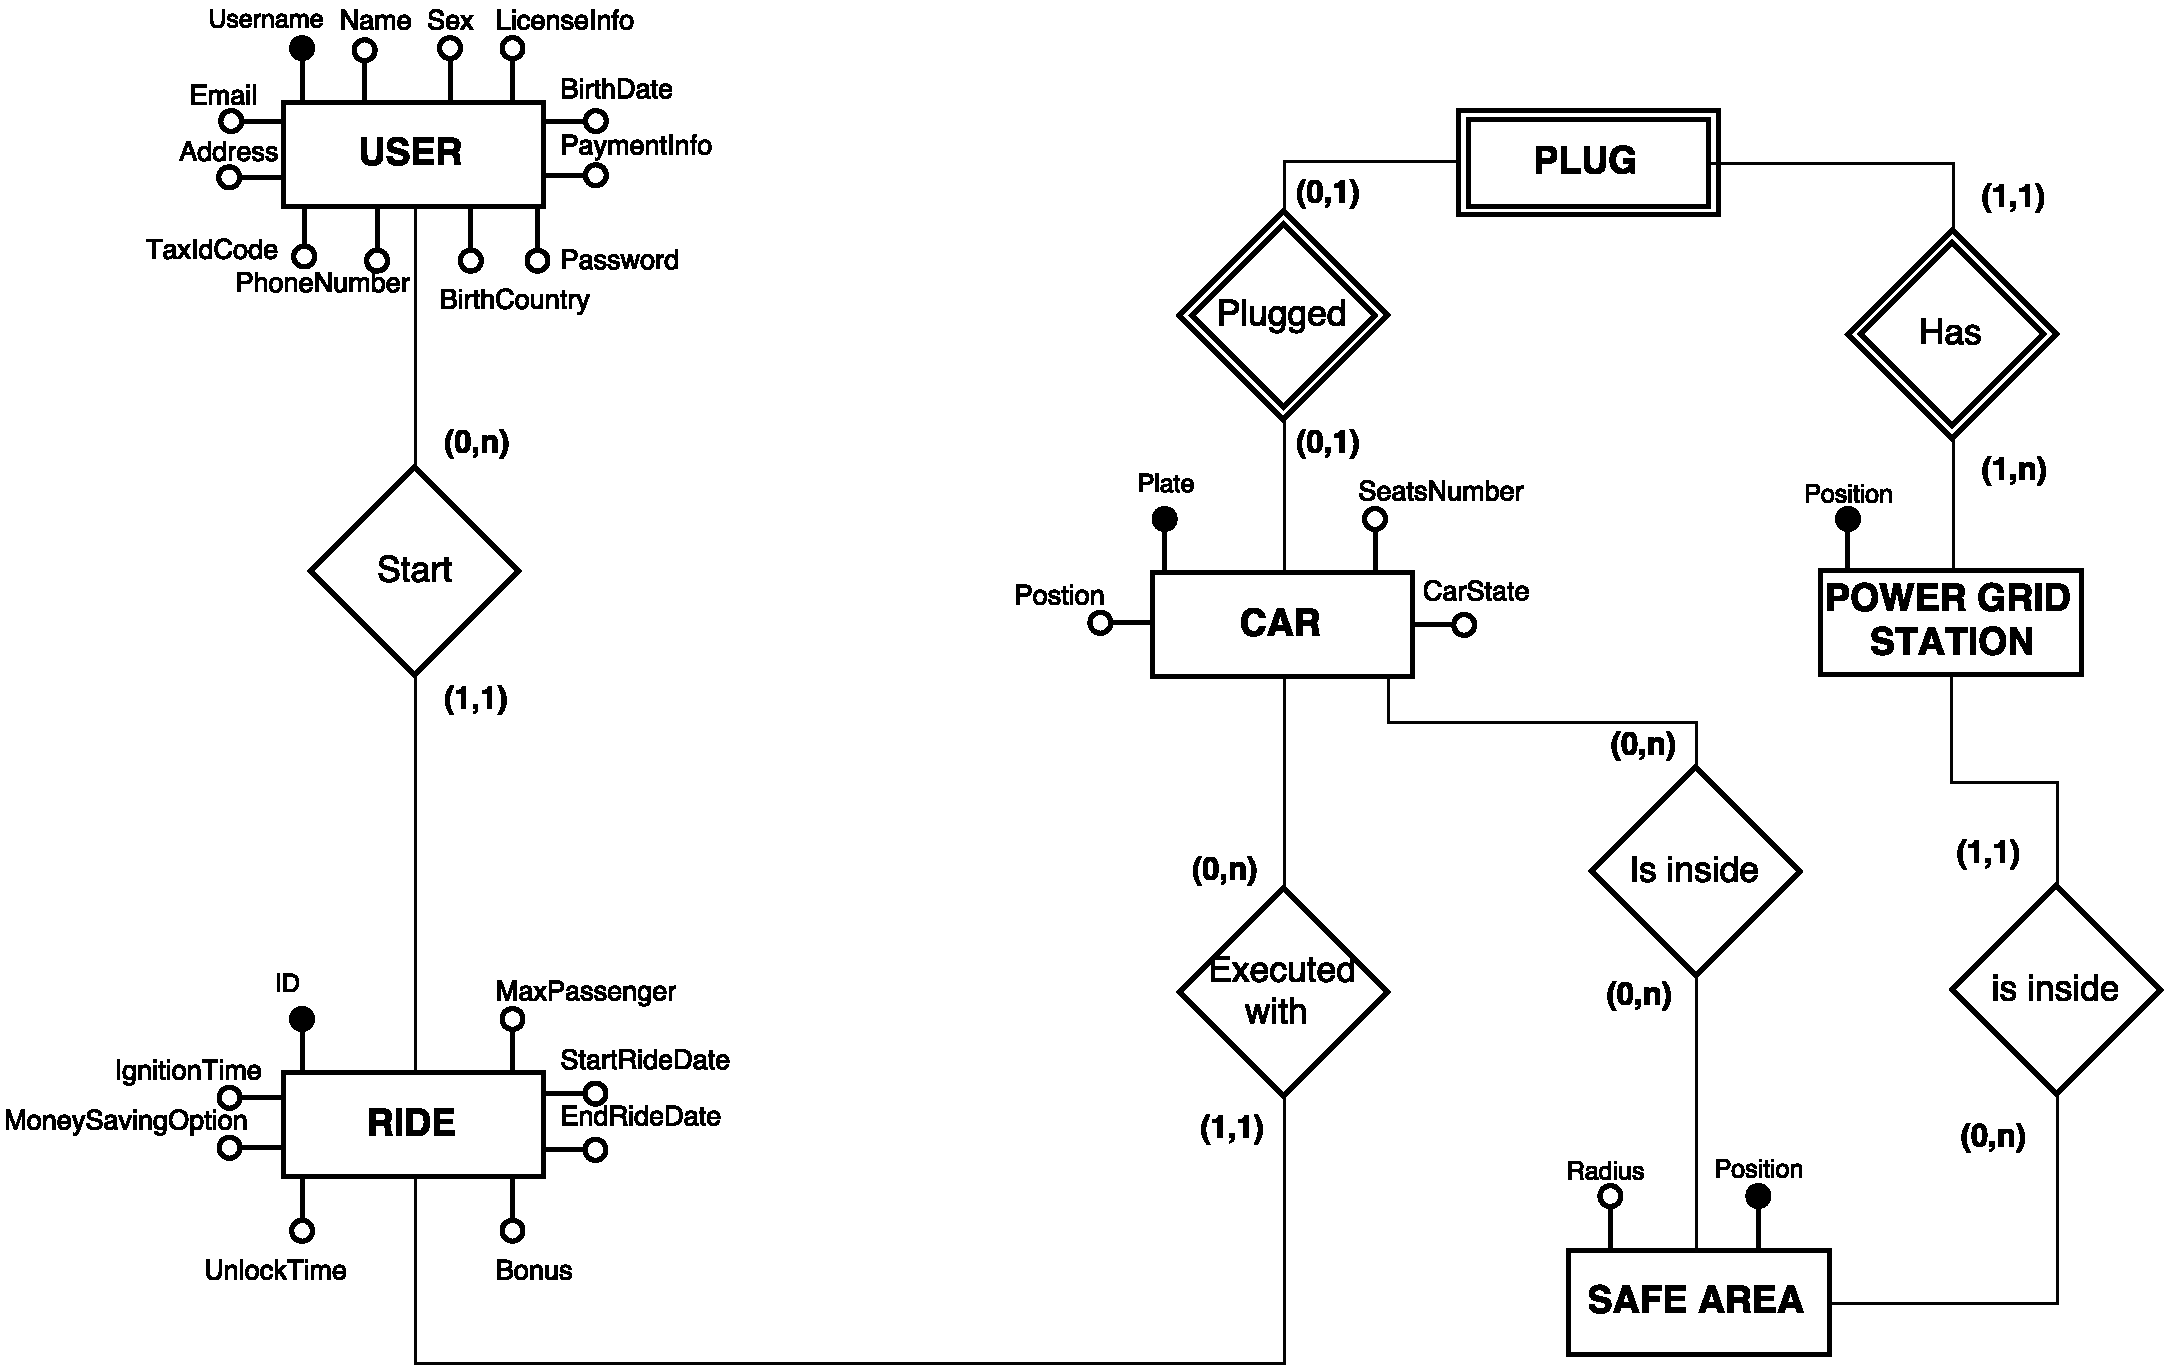
\includepdf{architectural_design/Architecture_Diagrams/ERDiagram.pdf}


